% =====================================================================
% 6.7 Precisão simples e precisão dupla
% =====================================================================
\subsection{Precisão simples e precisão dupla}
\label{sec:precisao}

A Figura~\ref{fig:prec} e a Tabela~\ref{tab:prec} repetem o RK4 do degrau, agora até 4~ms, em \emph{binary64} e \emph{binary32}. Enquanto o truncamento domina, as duas curvas coincidem: em \(h=8~\mu\mathrm{s}\) o erro é \(6{,}3\times 10^{-8}\)~A nos dois formatos. A partir de \(h=4~\mu\mathrm{s}\) a precisão simples descola e passa a oscilar entre \(3\times 10^{-8}\) e \(8\times 10^{-8}\)~A. Refinar mais o passo piora o resultado: em \(h=3{,}125\times 10^{-2}~\mu\mathrm{s}\) o erro sobe a \(4{,}35\times 10^{-7}\)~A. A precisão dupla continua a cair com inclinação 4 até \(3{,}08\times 10^{-16}\)~A, em \(h=6{,}25\times 10^{-2}~\mu\mathrm{s}\), e só então dá um passo para cima, para \(7{,}95\times 10^{-16}\)~A. O épsilon de máquina da precisão simples é \(1{,}19\times 10^{-7}\); o da dupla é \(2{,}22\times 10^{-16}\). O piso observado na corrente, cuja amplitude é de poucos centésimos de ampère, fica uma ordem abaixo do épsilon simples e junto do épsilon duplo no extremo do ensaio.

\begin{table}[htbp]
\centering
\caption{Erro máximo da corrente no RK4, em ampères, conforme o formato IEEE 754. Intervalo de 4~ms.}
\label{tab:prec}
\small
\begin{tabular}{@{}rrr@{}}
\toprule
\(h\) (\(\mu\)s) & \emph{binary64} & \emph{binary32} \\
\midrule
8{,}00 & \(6{,}32\times 10^{-8}\) & \(6{,}05\times 10^{-8}\) \\
4{,}00 & \(3{,}94\times 10^{-9}\) & \(2{,}82\times 10^{-8}\) \\
2{,}00 & \(2{,}46\times 10^{-10}\) & \(6{,}37\times 10^{-8}\) \\
1{,}00 & \(1{,}53\times 10^{-11}\) & \(4{,}07\times 10^{-8}\) \\
0{,}50 & \(9{,}58\times 10^{-13}\) & \(6{,}45\times 10^{-8}\) \\
0{,}25 & \(6{,}00\times 10^{-14}\) & \(8{,}19\times 10^{-8}\) \\
0{,}125 & \(3{,}76\times 10^{-15}\) & \(1{,}94\times 10^{-7}\) \\
0{,}0625 & \(3{,}08\times 10^{-16}\) & \(2{,}03\times 10^{-7}\) \\
0{,}03125 & \(7{,}95\times 10^{-16}\) & \(4{,}35\times 10^{-7}\) \\
\bottomrule
\end{tabular}
\fonte{Elaborado pelos autores (2026).}
\end{table}

\begin{figure}[htbp]
\centering
\caption{Erro do RK4 em precisão dupla e simples. O truncamento cai com o passo; o arredondamento da precisão simples estabelece um piso e, abaixo dele, o erro volta a subir.}
\label{fig:prec}
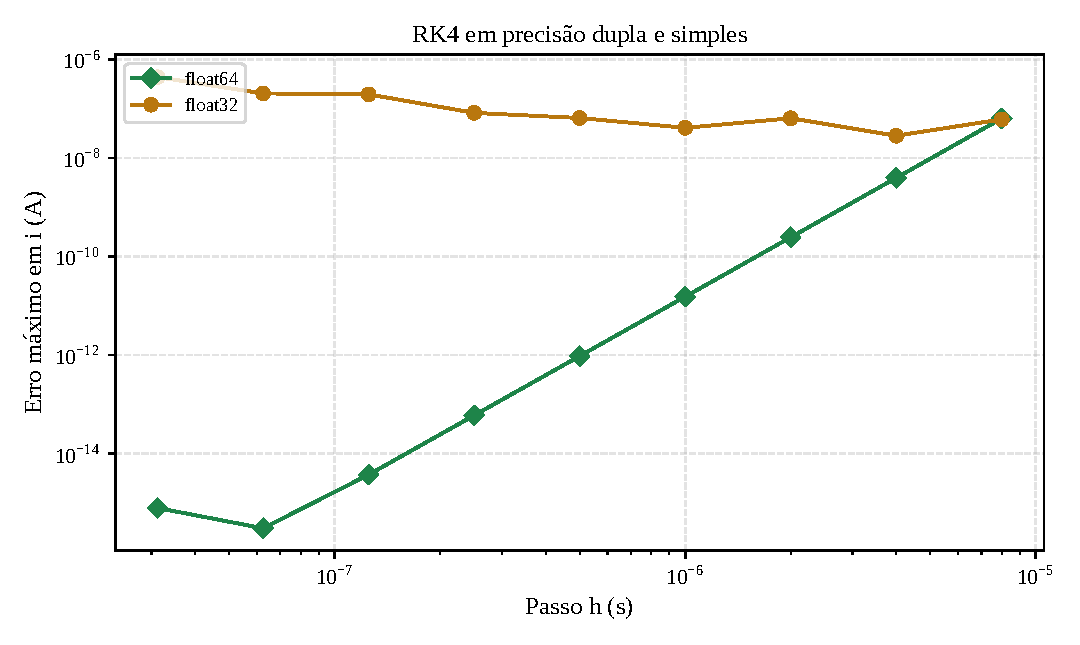
\includegraphics[width=0.92\textwidth]{precisao.pdf}
\fonte{Elaborado pelos autores (2026).}
\end{figure}

O número importa para um processador embarcado ou um DSP que só oferece ponto flutuante de 32 bits em hardware. Neste circuito, gastar um passo menor do que cerca de 1~\(\mu\)s em precisão simples não compra dígito nenhum. Uma corrente de dezenas de miliampères fica com erro absoluto perto de \(10^{-7}\)~A, o que é folgado para desenhar a forma de onda e pode ser curto para uma integração muito longa, para uma diferença de duas simulações próximas ou para um \(Q\) tão alto que a energia dissipada por ciclo seja comparável ao erro acumulado. Precisão dupla emula o formato largo em software, com custo de tempo. O ensaio quantifica o que se troca.
